\section{Experiments and Results}
\label{sec:experiments}

% introduction of task being studied and description of the demonstration dataset
We evaluate the greedy policy and two beam search lookahead policies using the Willow Garage PR2 robot, for the task of tying an overhand knot.
We use the set of demonstrations collected by \citet{Schulmanetal_ISRR2013} for their rope-tying experiments.
These demonstrations were collected in the real world and consist of 148 pairs of point clouds and gripper trajectories.
The point clouds were collected using an RGBD camera and then filtered based on color to remove the green background of the table, and leave only the point cloud representation of the rope.
The gripper trajectories were recorded kinesthetically, from human-guided demonstrations that move the robot's grippers to tie a knot.
The dataset contains demonstrations for the three steps of tying an overhand knot, as well as demonstrations to recover from rope states that could lead to failure cases.

The training, validation, and evaluation of the trained policy are run in simulation.
In simulation, the rope is represented as a linked chain of capsules with bending and torsional constraints using Bullet Physics~\cite{Bullet_Physics}.
To evaluate, we run the trained policy in simulation on randomly drawn initial rope configurations, and measure the success rate. We define success as tying an overhand knot in a sequence of 5 or fewer actions.
The initial rope states are perturbed configurations of randomly chosen initial rope states from the demonstrations.
The process of perturbing a rope state consists of selecting five uniformly-spaced points along the rope and dragging each in a random direction for a random radius of within 15 cm.
The randomly generated initial rope configurations mentioned hereafter are drawn from this distribution.

\subsection{Expert-labeled Examples}
For the labeled examples \labelset{} used to train our \mmql{} model, we distinguish between expert- (i.e. human-) labeled examples and automatically generated leave-one-out labeled examples.
Our expert-labeled examples consist of point clouds, each associated with the action that the expert human chooses for that point cloud.
The point clouds in these examples consist of sequences of complete task executions, from a randomly drawn initial rope configuration to a knot (Section~\ref{subsec:labeledex}.
%In particular, we simulate sequences of actions for various random initial rope configurations, with a human in the loop selecting the actions to achieve a knot-tie.
In practice, the expert does not select the optimal action for the current state among all the actions.
Instead, the actions are ranked in increasing order of registration cost with respect to the current state, since actions with smaller registration cost are more likely to succeed.

We evaluate the success rate of the proposed method under the following policies: greedy, one-step lookahead with width 10, and two-step lookahead with width 5.
For this evaluation, 1000 expert-labeled examples are used.
For each of these policies, the optimization hyperparameters $C$, $D$ and $F$ are first tuned via holdout validation, using a holdout set of 100 randomly drawn initial rope states.
Then the best-performing hyperparameters are used to calculate the weights and then run each of the three policies on the evaluation set, which consists of 500 randomly drawn initial rope states.
% TODO: Add in what the hyperparameters are, once we decide on them
As a baseline comparison, we also evaluate using the nearest neighbor policy presented in \citet{Schulmanetal_ISRR2013}.
Their policy chooses the action associated with the state that has the smallest bidirectional registration cost with respect to the current state.
The success rates obtained under these policies are summarized in Table~\ref{table:performance}. Note that our best results surpass the baseline by XX\%.
% TODO: Add more analysis of the results, e.g. 1-10 and 2-5 lookahead perform approximately equally well

\begin{table}
  \centering
  \begin{tabular}{lc}
    \toprule
      Policy & Test Accuracy\\
    \midrule
      Nearest neighbor \cite{Schulmanetal_ISRR2013} & XX\% \\
    \midrule
      Greedy & XX\% \\
      Lookahead (depth 1, width 10) & XX\% \\
      Lookahead (depth 2, width 5) & XX\% \\
    \bottomrule
  \end{tabular}
  \caption{Success rate of tying an overhand knot under different policies.}
  \label{table:performance}
\end{table}

The approximate values of the states for the 500 evaluated runs in the validation set are plotted in Figure~\ref{fig:values} as a function of time steps 1 through 5.
%TODO: shift plot from 1 to 5
Observe that the state values are generally increasing; we expect this since the Bellman constraints in our formulation pushes states closer to the goal to have higher values.
Also, recall that the state value of the tied knot is close to zero, which is visible in the figure (Equation~\ref{eq:bellman_goal_constr}).
For most of the runs, the policy is able to reach the goal state in 3 steps, which is optimal since the expert took a minimun of three actions to tie a knot.

\begin{figure}[h!]
  \centering
    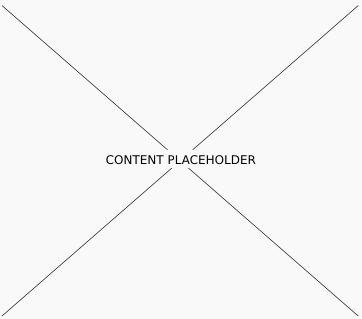
\includegraphics[width=0.9\linewidth]{figures/placeholder.png}
  \caption{State values as a function of time steps}
  \label{fig:values}
\end{figure}

We also study the relation between the number of expert-labeled examples and the success rate for each of the four policies, including the nearest-neighbor baseline policy.
These success rates are shown in Figure~\ref{fig:number_examples}.
The success rate of the baseline policy is a constant, since the nearest neighbor policy doesn't use the expert-labeled examples.
As expected, the success rate increases as more labeled-examples are used.
%TODO: Mention that there are diminishing returns as you increase the number of expert examples (I assume the graph will look like that)

\begin{figure}[h!]
  \centering
    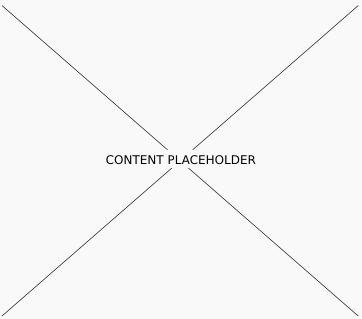
\includegraphics[width=0.9\linewidth]{figures/placeholder.png}
  \caption{Success rates as a function of the number of expert-labelled examples for the four policies}
  \label{fig:number_examples}
\end{figure}

\subsection{Leave-One-Out Labeling}

We now evaluate the performance when training on leave-one-out labeled
examples, as outlined in Section~\ref{subsec:lool}.

After holdout validation and evaluation, done in the same manner as our main
experiment, we find that using a leave-one-out labeled example set achieves a
performance of XX\%, a drop of XX\% from our supervised result.
%\et{It feels difficult to do further analysis without an actual number here. I'll save this
%for later, if that's alright with everyone.}
